\chapter{Implemention}
	To develop a system that uses Image Processing to get data from token patterns via a webcam into Unity and \textit{"translate"} it into a Virtual Reality garden that can be explored through the HTC Vive using Steam VR, there are many considerations that have to be made. This section explains the program implementation and some of the algorithms that went into the development process. Furthermore, some of the most essential and relevant code snippets will also be presented.
	
	\section{VR in Unity}
	When discussing the initial idea at the semester workshop it was suggested that we implement the design in the Unity game engine\footnote{Unity's homepage \url{https://unity3d.com/}}. Unity allows high-level management of objects in space, and would reduce development time on all the non-image processing based parts by inconceivably many hours.
	\todo{Describe technical details of VR in Unity using Steam VR}
	
	\section{DLLs and Unity}
 		Unity has a fair number of different options for performing image processing. We would be creating the fiducial markers from scratch and could not use any preexisting software. At this point, we were already familiar with OpenCV, a fast library for image processing and computer vision, so developing using OpenCV made sense.\\
 		
		One issue is that Unity uses C\# but OpenCV is only developed for C++, C, Python, and Java. The method used in this project to bridge this language barrier is to compile the C++ code as a DLL, or \textit{"Dynamic-link Library"}, and import it into the C\# code. DLLs cannot be executed in the way normal applications are, and instead can be used by other applications. Because they can be complied from a host of different languages they are not limited to what C\# code can do. Another advantage is that they are compiled in machine code and are therefore very fast\footnote{How to Write Native Plugins For Unity \url{https://www.alanzucconi.com/2015/10/11/how-to-write-native-plugins-for-unity/}}. There are some drawbacks to using DLLs as well, and these brought on some challenges during the implementation. Firstly, passing an object between the DLL and Unity is difficult because Unity cannot understand the same code as in the plug-in. On the C++ side you do not have a terminal, which means that getting any information about what is happening inside the DLL for debugging purposes is very problematic. For the same reason, debugging crashes is tricky, and the program would often crash without any feedback. Listing \ref{listing:dllExport} shows how to declare a function for export in C++.
\begin{listing}[H]
\caption{How to declare a function for DLL export in C++}
\label{listing:dllExport}
\begin{minted}[frame=lines, framesep=2mm,baselinestretch=1.1,fontsize=\footnotesize,linenos]{cpp}
extern "C" __declspec( dllexport ) int init(int w, int h);
\end{minted}
\end{listing}
\codeword{extern "C"} tells the compiler to not change the function's name, so that it can be imported into Unity. \codeword{__declspec()} tells the linker to do something depending on the argument, which in this case is \codeword{dllexport}. This lets the compiler know that it should export a function to a DLL. So now the function will be exported under a name that we know. In Unity a corresponding \codeword{DllImport("name")} will be used to import the function in Unity. Listing \ref{listing:dllImport} shows how this looks in C\# on the Unity side.
\begin{listing}[H]
	\caption{How to declare a function for DLL import in C\#}
	\label{listing:dllImport}
	\begin{minted}[frame=lines,
	framesep=2mm,baselinestretch=1.1,fontsize=\footnotesize,linenos]{cpp}
[DllImport("unityOpencvPlugin", EntryPoint = "init")]
public static extern int Init(ref int outCameraWidth, ref int outCameraHeight);
	\end{minted}
\end{listing}
The name of the DLL file "unityOpencvPlugin" is given, and the function that we want to import is the "entrypoint". Unity will then do a search for a function called \codeword{init} in the DLL "unityOpencvPlugin". Here it is important that the methods names match completely, otherwise it will not be found. In line 2, a function is declared that will call the imported method. Note that this function must have the same signature (return type and arguments). Unity can not check whether or not this is true, so it will proceed as if it is the case. Signature compatibility is sensible for primitive types like \codeword{int}, but for objects it becomes a bit trickier. To do so requires declaration of similar objects in both languages, with variables in the same order, otherwise the data will not make sense when returned. In our case we need to return the markers found after image processing. They are represented in a structure like shown in Listing \ref{listing:objects}. 
\begin{listing}[H]
	\caption{Objects in C\# and C++}
	\label{listing:objects}
	\begin{minted}[frame=lines, framesep=2mm,baselinestretch=1.1,fontsize=\footnotesize,linenos]{c++}
//in C++
struct ObjectData {
   int X, Y, Type, RotationX, RotationY, Rotation;
};

//in C#	
[StructLayout(LayoutKind.Sequential, Size = 24)]
public struct CVObject{
   public int X, Y, Type, RotationX, RotationY, Rotation;
}
	\end{minted}
\end{listing}
In Unity the structure needs to be laid out sequentially when exported to unmanaged memory\footnote{Unity layout \url{https://msdn.microsoft.com/en-us/library/system.runtime.interopservices.layoutkind(v=vs.110).aspx}}. We are going to be returning several objects. One for each token. In this case it is easier to pass a pointer to an array, and make C++ fill it out from the code. A few things are needed for this to work. The function needs to take a reference as an argument and the size of the array must be passed as an argument. Otherwise the function might try to access data outside of the array. The memory being referenced must also remain static or the pointer would no longer point to the right data. In C\# the keyword \codeword{Fixed} prevents data from being moved in memory, and \codeword{unsafe} enables working with pointers. In Listing \ref{listing:pointer} below there is an example from our implementation in the project where we pass a pointer to C++. %be careful with "unsafe" though. It oftentimes leads to children. 
\begin{listing}[H]
\caption{The function call to pass a pointer to C++, which is filled with object data by the code}
\label{listing:pointer}
\begin{minted}[frame=lines,
		framesep=2mm,baselinestretch=1.1,fontsize=\footnotesize,linenos]{c++}
unsafe{
	fixed (CVObject* outMarkers = _markers){
		Cap(outMarkers, _maxMarkerDetectCount, ref detectedMarkersCount);
	}
}
\end{minted}
\end{listing}
\section{Implications of working in VR}
Virtual Reality is computationally demanding. In 2016 Nvidia estimated that an immersive VR experience was seven times more demanding than PC gaming\footnote{www.forbes.com : \url{goo.gl/AFsBGs}}\footnote{www.pcgamesn.com : \url{https://goo.gl/5Rzy41}}. Nvidia got the number by combining the resolution needed for VR, 2 times 1680 x 1512, with the frame rate needed to avoid the adverse effect of VR, 90 fps. They compared the numbers with the same requirements for pc gaming 1920 x 1080, and 30 fps. However, this group agrees that 45 fps is closer to the minimum for a smooth experience, which still leaves the average laptop way underpowered. At 45 fps compared to VR it has to render 2.5 times as many pixels, and twice as many frames per second.
For this reason the algorithm should be fairly quick to execute, because there is going to be quiet a load on the system running the VR experience. Consequently, we have been trying to optimize our algorithm.

\section{BGR to RG chromaticity conversion}
Since we are now diving into image processing, we can show the outputs of the operations. A snap shot from the prototype's webcam has been taken for just this purpose is shown in \autoref{fig:snapshot}, and after each of the image processing sections the output will be shown.
\begin{figure}[H]
\centering
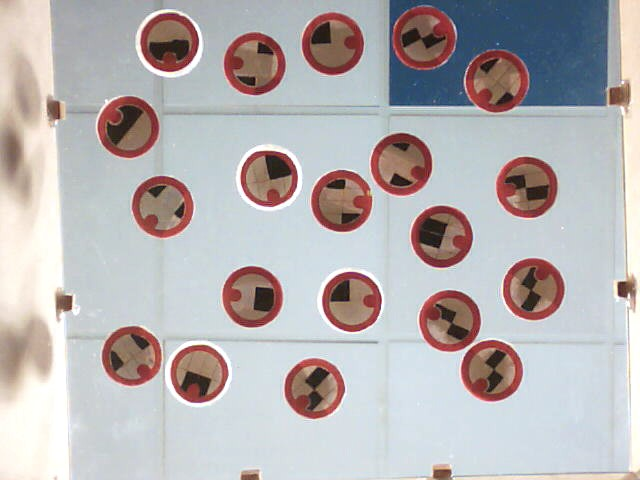
\includegraphics[width=0.6\linewidth]{figure/Analysis/testimage.jpg}
\caption{A test image that will show the results of the image processing}
\label{fig:snapshot}
\end{figure} 
It was found that differences in lighting conditions made thresholding the feed from the camera at best suboptimal. To circumvent this the feed is converted to RG chromaticity\footnote{Wiki page for RG Chromaticity: \url{https://en.wikipedia.org/wiki/Rg_chromaticity}}, also known as normalized RGB, and henceforth RG. RG contains no intensity information and as such is not a color space but instead a chromaticity space\footnote{Wiki page for Chromaticity: \url{https://en.wikipedia.org/wiki/Chromaticity}}.
\subsection{Theory of RG}
The critical property that RG has is that it does not record the individual channels intensity, but rather the color's intensity as a percentage of the total intensity. Mathematically the RG value of a channel can be derived from an RGB value in the following way.
\[ RG_x = \frac{RGB_x}{RGB_1 + RGB_2 + RGB_3}\]
Where $x$ represents which of the channels that is to be converted. This will give a value between 0 and 1 depending on how big a percentage of the total intensity comes from that particular color. Since floats are operationally slow, it is advised to scale the value to 8bits by multiplying by 255. So instead of operating on a range of 0,000 to 1,000, it operates on a range og 0 - 255. If one were to convert all three channels, with capital letter representing the RG chromaticity, the channels can be found as.
\[ RED = \frac{red}{red + blue + green} * 255\]
\[ BLUE = \frac{blue}{red + blue + green} * 255\]
\[ GREEN = \frac{green}{red + blue + green} * 255\]
This means that in RG the sum of all channels must be 255.
\[ \frac{red}{red + green + blue} + \frac{green}{red + green + blue} +  \frac{blue}{red + green + blue} =  \frac{red + green + blue}{red + green + blue} = 1\]
It is observed that in RG the channel values are codependent. If the value of red is large, then the other channels must by definition contain small values as they all must add up to 255. A result of this is that one can find the value in one channel if the other two are known.
\[ BLUE = 255 - RED - GREEN\]
So it is possible to store the data using two bits, and calculate the third color if it is needed. This loss of information comes from the loss of intensity data\cite{NormRGB}. For example, two colors (0,10,50) and (0,50,250) will produce exactly the same values when converted to RG. 
\[ BLUE = \frac{50}{50 + 10} * 255 = (int)212.5 = 212 \]
\[ BLUE = \frac{250}{250 + 50} * 255 = (int)212.5 = 212 \]
The resultant colors can be seen in figure \ref{fig:conversion} The same is true for any two color that are proportionately similar.\\
\begin{figure}[H]
	\centering
	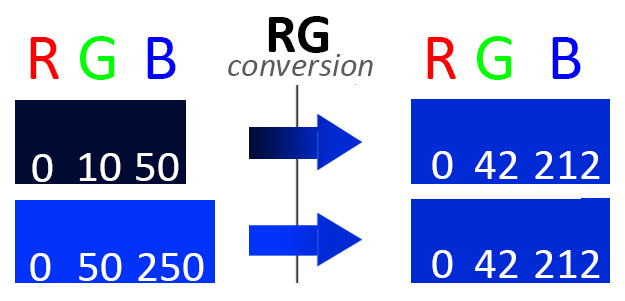
\includegraphics[width=0.6\linewidth]{figure/Analysis/rgconversion.png}
	\caption{Two colors of very different intensity are identical when converted to RG because they have the same percentages of the different colors. This make the RG color space more resistant to different lighting condition}
	\label{fig:conversion}
\end{figure} 
In relation to image processing one has to be aware that noise, particularly in shadows, mess with the rg space. For this reason it is recommended to zero the values if the total sum is below a certain value.

\subsection{rg chomaticity in code}
The process of converting an rgb image described above is a matter of simple point processing. We have made a few changes to speed up the process at runtime. The current code performs these two steps at each pixel in the input image.\\
\begin{enumerate}
	\item Find the sum of the rgb chanels.
	\item Assign the corresponding pixel in the output to the value found in a look up table using the sum and value in the channel\\
\end{enumerate}
Really the only big change is the decision to use a look up table. A look up table is useful if you are going to be performing the same operation on similar data a lot of times. 
\subsection{Lookup tables}
The concept of a lookup table is, "instead of calculating this thing every time, why don't i calculate a table with the results of all possible inputs and just look up what the result is". This might sound like madness until one realizes the magnitude of data we are working with. The webcam that we used had a resolution of 640 x 480. That is 307200 pixel. Now multiplications and additions are very fast, but division is a more expensive operation and we have to do division and multiplication three times per pixel (one for each channel). We found that at runtime using a look up table increased the speed of our conversion algorithm by 100.25\% as can be seen in table \ref{table:rgConvSpeed}.\\
\begin{multicols}{2}
	\begin{figure}[H]
	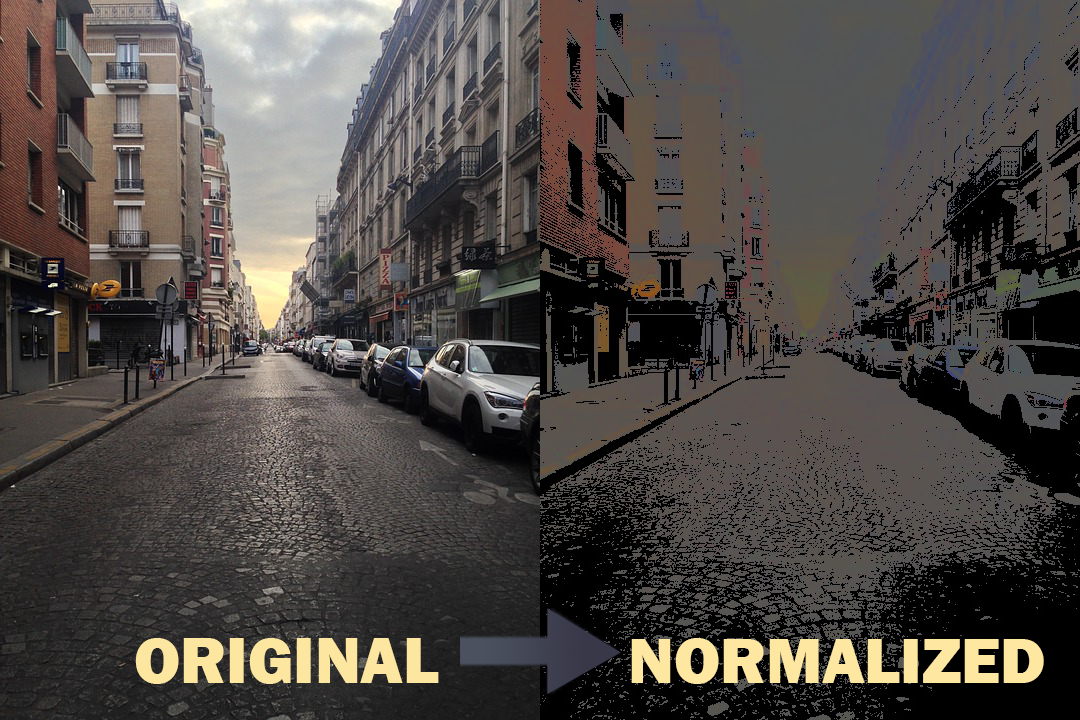
\includegraphics[width=1\linewidth]{figure/Analysis/Normalized.png}
	\label{rgConversion}
	\caption{Test image used to test the speed of the BGR to RG conversion. Using a look up table halved it execution time}
	\end{figure}

    \columnbreak
	\begin{table}[H]
		\centering
			\caption{Time taken to run the function. It can be seen that more data precomputed into a lookup table, results in faster execution. Due to the number of repetitions even something as basic as an "if smaller than" statement can significantly increase the speed. Times are average times after 100000 runs on a test image with the dimensions 540 * 720}
		\begin{tabular}{ l | l }
			\hline			
			No lookup table & .0015028 sec\\
			Look up if above threshold & .0010218 sec\\
			Look up table always& .0007741 sec\\
			\hline 
		\end{tabular}
	\label{table:rgConvSpeed}
	\end{table}
\end{multicols}

\subsection{Creating a look up table}
Creating a look up table is straight forward. You take the operation that would be performed, and save the results for the range of inputs needed. We know from the theory section that a color can be assigned by $RGcolor = 255 * \frac{color}{sumOfColor}$. There are two variables at play here. Sum which can vary between 0, when all colors are zero, and 765, and Color which can vary between 0, and 255. To compute a lookup table  that includes all possible combinations of variables, we need an array of size 766 * 256. The values are assigned when creating the table using a double for loop, as can be seen in Listing \ref{listing:lutTable}.
\begin{listing}[H]
\caption{Instantiating our lookup table}
\label{listing:lutTable}
\begin{minted}[frame=lines,
	framesep=2mm,baselinestretch=1.1,fontsize=\footnotesize,linenos]{c++}
	int divLUT[766][256]; //division lookuptavle;
	for (int i = 0; i < 766; i++) {
		for (int j = 0; j < 256; j++) {
			if (i < rgConvThreshold) { 
				divLUT[i][j] = 0;
			}
			else {
				divLUT[i][j] = (j * 255) / i;
			}
		}
	}
\end{minted}
\end{listing}
The first thing the loop does is to check if the arguments are below the threshold where they should be zeroed (to prevent noise in dark areas from messing with the image). In that case it sets the index to zero. Otherwise calculate the value that would result from the color(j) divided by sum(i) and multiplied by 255.
\subsubsection{Suming rgb channels and looking up results}
This is point processing and as such it calls for a double for loop to ensure each pixel is visited. The function takes an input image assumed to be BGR, and an output image also amused to be BGR. The ampersand(\&) in the function signature, seen in Listing \ref{listing:sum}, indicates that the argument should be passed by reference. This allows for changes to the original data to be made. If not included we would be making changes copies instead.\\\\
Before the loop we instantiate three pointers so we don't have to instantiate them inside the loop. \codeword{p} is a pointer to a row in the rgb image we want to convert. \codeword{cp} is a pointer to the equivalent row in the output image. \codeword{lutptr} points to a row in the look up table. This is useful because the sum, and therefore the column, will be the same for each color in the pixel. So we will be looking at the same row three times in a row, one for red, one for blue, and so on. With the pointers one will not have to jump as far in memory every time the lookup table is used. Basically, it is quicker to get from \codeword{lutptr[sum][0]} to \codeword{lutptr[sum][red]}, then from the start to \codeword{lutptr[sum][red]}. 
\begin{listing}[H]
	\caption{RG conversion code}
	\label{listing:sum}
	\begin{minted}[frame=lines,
		framesep=2mm,baselinestretch=1.1,fontsize=\footnotesize,linenos]{c++}
void preLookUpBgr2rg(Mat &in, Mat &out, uchar (&divLUT)[766][256]) {
	//declare other variables
	int nCols = in.cols * 3;	//since there's 3 channels per pixel
	
	for (int i = 0; i < nRows; i += GRIDSIZE) {
		p = in.ptr<uchar>(i);
		cp = out.ptr<uchar>(i);
		
		for (int j = 0; j < nCols; j += 3 * GRIDSIZE) {
			blue = p[j];
			green = p[j+1];
			red = p[j+2];
			sum = blue + green + red;
			lutptr = divLUT[sum];
			//cp[j] = *(lutptr + blue);  not needed
			cp[j + 1] = *(lutptr + green);
			cp[j + 2] = *(lutptr + red);
		}
	}
}
	\end{minted}
\end{listing}
Inside the for loop, the code starts by saving the values of each channel to the corresponding variables. The values are then added together. Now we have the two variables that we need to use the lookup table. Since the sum is not going to change we get the address of the row of the sum and save it in \codeword{lutptr}. Now we can assign the values using \codeword{lutptr}. In accordance with the theory section blue is unnecessary data and so does not need to be assigned. We will be calculating the blue when showing the  output, but that is only to make the image less jarring for humans to look at. In the final code it \label{key}can be omitted. After executing the function on our test image the following Figure \ref{fig:rgsnapshot} is the output.
\begin{figure}[H]
	\centering
	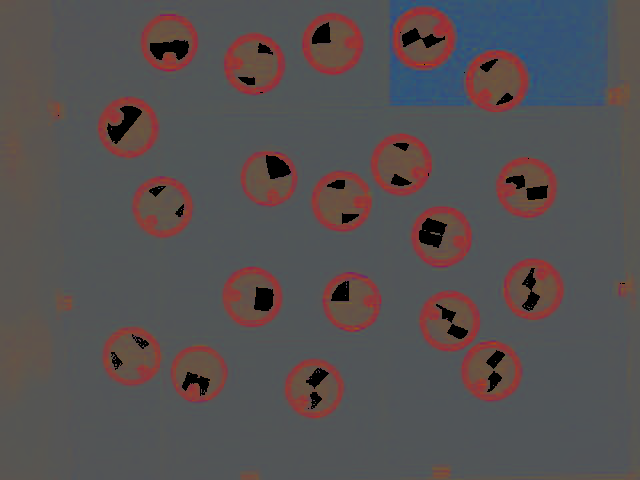
\includegraphics[width=0.6\linewidth]{figure/Analysis/rgbNorm.png}
	\caption{Test image after being converted into RG}
	\label{fig:rgsnapshot}
\end{figure} 

\section{Thresholding in RG}
\todo{write a bit more about the implication of each threshold}
Because RG can be represented by two values it is possible to plot the  chromaticity space using two axes, as can be seen in figure \ref{fig:rgbNorm}. The image contains a slightly modified, but prettier, RG space. 
\begin{figure}[H]
	\centering
	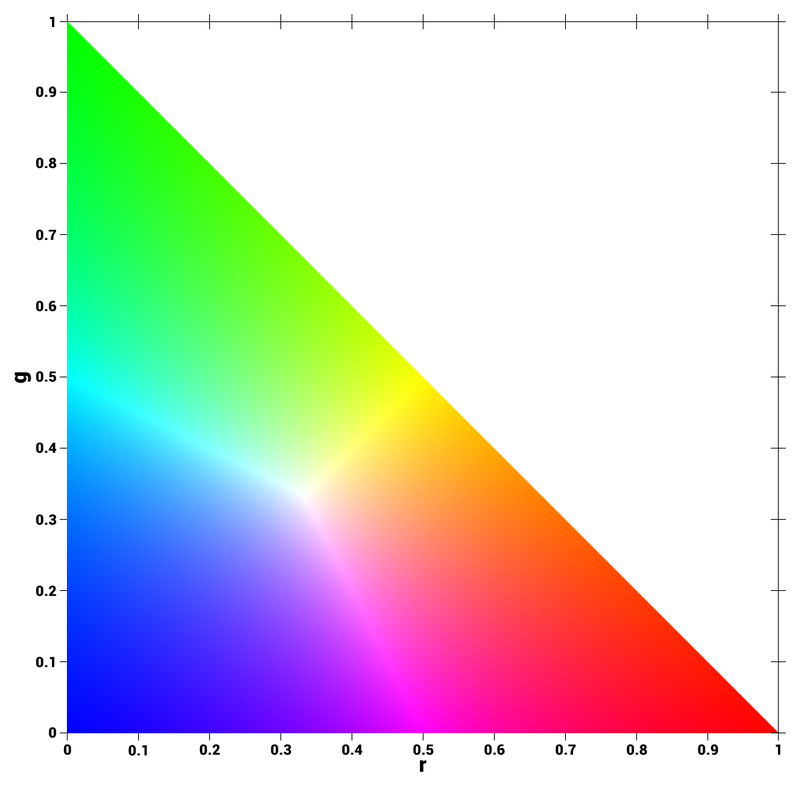
\includegraphics[width=0.5\linewidth]{figure/Analysis/normRGB.png}
	\caption{The entire RG color space is visible here, it can be represented in 2D due to the loss of intensity data that happens during conversion. Image from \url{https://en.wikipedia.org/wiki/Rg\_chromaticity}, made by Vampyrium, and will be used to illustrate the results of different thresholds. Under the CC BY-SA 3.0 license.}
	\label{fig:rgbNorm}
\end{figure}
There are different ways to threshold in RG, and because of the two dimensionality they are wonderfully reminiscent of high school math. Common amongst all of the presented approaches is that they use the red and green values of each pixel to determine whether the pixel should be set to 255
or 0.\\\\
\textbf{In range}, is an often used way of thresholdnig in the HSV color space\footnote{\url{https://docs.opencv.org/3.2.0/df/d9d/tutorial\_py\_colorspaces.html}}. One sets a range in each axis in which to threshold. For example between 160 to 255 in red, and 0 to 60 in green. The thresholding consists of comparing the red and green value in each pixel to the ranges. If both values are inside the designated range the pixel is set to 255, else it is set to 0. The resulting threshold can be seen in \autoref{thresholdintrange}. This will create a square segmentation in the chromaticity space. It should not surprise anyone because we are comparing two constants. Constants create straight lines. With its square shape, it can be difficult to get a broad enough spectrum, without cutting into different colors. For example, under blue light from the sky the markers might be a fair bit bluer. You also cannot set it too wide, since doing so will cause white things to also be segmented. There are ways the provide more control over the segmentation.\\
\begin{multicols}{2}
	\begin{figure}[H]
		\centering
		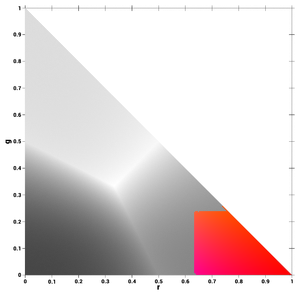
\includegraphics[width=1\linewidth]{figure/Analysis/inrangethresholdcolor.png}
		\caption{in range threshold in rg space}
		\label{thresholdintrange}
	\end{figure}
	\columnbreak
	\begin{figure}[H]
		\centering
		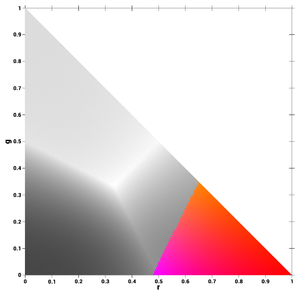
\includegraphics[width=1\linewidth]{figure/Analysis/belowlinethresholdthresholdcolor.png}
		\caption{below line threshold in rg space}
		\label{fig:thresholdbelowline}
	\end{figure}
	
\end{multicols}

\todo{we are now using below line and distance make accoridng changes}
\textbf{Line threshold}. Is another potential way to threshold. One creates a straight line with a formula $y = ax - b$. Where y and x each represent the two axes. $a$ determines the slope of the line and is controlled by $x$ which is one of the color. In this case, lets say $x$ is red. $b$ decides where the thresholding should start and can be found using $b =- i * a$. Where $i$ is the start point of the line. Based on the equation we can find value of green that would place it on the line for a given red value. Then our values can be compared the line to see which side of the line it is on. If the values are on the right side it to 255, else set it to zero. An example of this is a below line threshold as seen in \autoref{fig:thresholdbelowline}\\
\begin{multicols}{2}
	\begin{figure}[H]
		\centering
		\label{thresholddist}
		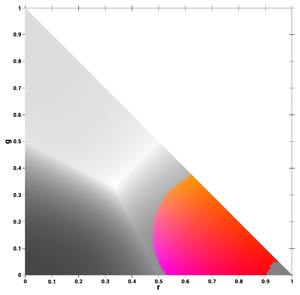
\includegraphics[width=1\linewidth]{figure/Analysis/distthresholdcolor.png}
		\caption{distance threshold in rg space}
	\end{figure}
	
	\begin{figure}[H]
		\centering
		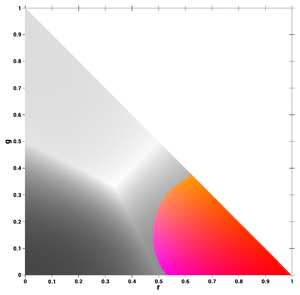
\includegraphics[width=1\linewidth]{figure/Analysis/thresholdcolor.png}
		\caption{combined threshold in rg space}
		\label{fig:threshold}
	\end{figure}	
\end{multicols}
\textbf{Distance threshold}. Is based on finding the chromaticity distance from the a pixels color to a reference value in RG. If the distance is below a threshold the set it to 255, else 0. In two dimensions the distance between two points, $p_0$ and $p_1$, can be found as $d = \sqrt{(p_1x - p_0x)^2 +(p_1y - p_0y)^2}$. In our implementation we used a distance threshold with a red value of 180 and a green value of 40 for our reference color. The threshold distance was set to 60. This produces the threshold observed in \autoref{fig:threshold}. There is a problem though. We are unable to threshold extremely red color.\\\\
\textbf{Combined Threshold}. It is possible to combine these different approaches to thresholding. Combining and subtracting the thresholds allows us shape the threshold as we want. Following the problems with segmenting extreme reds, we decided to put an in range on top of the distance based threshold to ensure that we could capture all the shades of red. The resulting threshold can be seen in \autoref{fig:threshold}. We found that this produces the most consistent threshold, and was the most resistant to lighting changes.

\subsection{Thresholding implementation}
Like the RG conversion this operation involves visiting each pixel once and performing an operation that uses its color values as inputs. You feel that, that is my look-up-table-senses tingling. Turning the equation into code is quiet simple. The operation that we need to perform is find the distance, if it is smaller than the threshold  set pixel to 255, else if larger than  else 0. How we initialized our table can be seen in listing \ref{listing:thresholdDist}.\todo{we have a new threshold}

\begin{listing}[H]
	\caption{Instantiating the Distance threshold look up table}
	\label{listing:thresholdDist}
	\begin{minted}[frame=lines,
framesep=2mm,baselinestretch=1.1,fontsize=\footnotesize,linenos]{c++}
uchar lookup[256][256];
for (int i = 0; i < 256; i++) {
	for (int j = 0; j < 255; j++) {
		if (j > 180) { // if red is above 180
			lookup[i][j] = 255;
		}else if (((i - g)*(i - g) + ((j - r)*(j - r))) < 3600) {
			lookup[i][j] = 255;
		}else {
			lookup[i][j]= 0;
		}
	}
}
\end{minted}
\end{listing}

Inside the double for loop there is an if statement that test the distance from the inputs $f(j,i)$ to a reference point $p(r,g)$. Rather than comparing it to the distance, it compares to the distance squared. This saves us having to use a square root. So we test if the distance is smaller than 60. If true make the index white, otherwise make it black. 
In terms of implementations using the lookup table, it is very similar to the rg conversion and as such it not worth mentioning. The output after thresholding the normalized test image, can be seen in Figure \ref{fig:thsnapshot}\\
\begin{figure}[H]
	\centering
	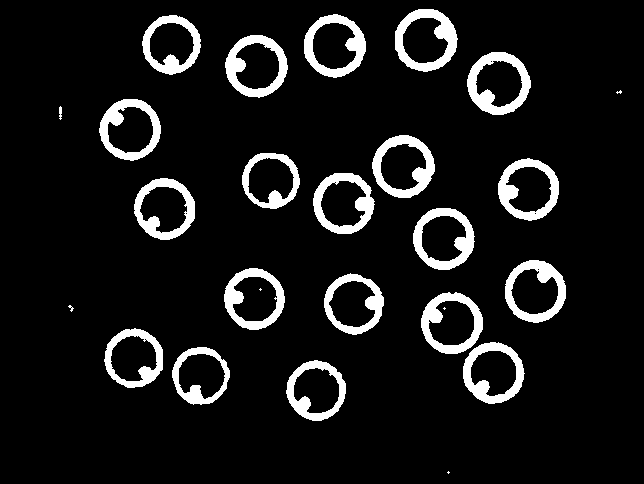
\includegraphics[width=0.6\linewidth]{figure/Analysis/thresholded.png}
	\caption{The thresholded version of out normalized test image}
	\label{fig:thsnapshot}
\end{figure} 
The algorithm has now produced a binary thresholded image with value that are either 255 or 0. This image is used to to a grassfire blob detection. 
\section{Blob detection}
Blob detection used to segment a picture into individual blobs. If you need to deal with multiple object in a image, it is worth investigating. 
\subsection{What is a blob, and why detect them}
Blob stands for \textbf{B}inary \textbf{L}arge \textbf{OB}ject. They represent regions of interest(ROI) in a image. Extracting the blobs from an image can significantly cut down on processing time, because the program now only have to process the ROI instead of the entire image. Another use is to calculate features that might be useful to know about the blob, like size, and bounding box, and a host of others. For a program a program trying to recognize real life objects, Knowing the range of features that the object normally produces can help it determine if a blob is that object. Generally these features are calculated from a list of pixels in the blob.\\\\
There is staggeringly large amount of features that could be calculated on a blob. But our job is made \textbf{A LOT} easier by three factors. First, our marker are resting on a surface perpendicular to the camera. This means that rotation will only happen in two dimensions and that the shape of the markers will not change substantially when rotated. Secondly, our markers are circles. There are many things to love about circle, their heigth/with relationship is the same in any rotation, and you can work with its radius. Finally, we are segmenting based on a color(red), and after the segmentation we are already left with mostly regions of interest(see Fig \ref{fig:thsnapshot}). Meaning our blob detection has to do less work in discriminating the blobs.
\subsection{The blob object and parameters}
The list of pixels and blob parameters are often held in an structure.
We created one for this purpose. Our blob structure is called \codeword{gylphObj}, because the pattern underneath can resemble a glyph\footnote{\url{goo.gl/HkFksM}}. The structure is declared as shown in listing \ref{listing:glyph}
\begin{listing}[H]
	\caption{The declaration of glyph object, the structure that contain a blob, as well has the parameters about it}
	\begin{minted}[frame=lines, framesep=2mm,baselinestretch=1.1,fontsize=\footnotesize,linenos]{c++}
		struct glyphObj {
			vector<cVector> list;
			cVector bBoxStart;
			cVector bBowEnd;
			cVector center;
			cVector rotation;
			int nr;
			bool returnable = false;
		};
	\end{minted}
	\label{listing:glyph}
\end{listing}
We dive deeper into the parameters and what they are used for in the next section, so the uses of the variables will be not discussed in detail here. However a brief overview is provided. 
cVector, short for coordinate vector, contains two int. One for each the dimensions. In c++ vector is a list type that can grow dynamically. So the vector of cVectors is going to contain the coordinates of all the pixels in the blob. bBox is short for bounding box and are the two coordinates used to draw a bounding box around the blob, and find its height to width ratio. Since a circle always has similar height to width ratio in any rotation, this parameter can be used to disqualify a lot of blobs. \codeword{center} is the coordinates to the center of the bounding box.
The integer \codeword{nr} is used to help visualize the grass-fire algorithm, and will later contain the found value from the pattern underneath the markers. Finally, since we find way more blobs than there are actual markers, and returning all the blobs to unity be a waste of time, a boolean \codeword{returnable} exists. It is only set to true if the blob passes all test and therefore is considered a marker.
\subsection{Blob Extraction by recursion}
All features of a blob are calculated from a list of pixels included in it. This section deals with how to get that initial list of pixels. In a segmented image, a blob is nothing more than a number of white pixel with other white pixels as neighbors. Because of this property each pixel in the blob must be connected to each other pixel through a string of white pixels. Correspondingly, a blob can be found by finding all connected pixels of any pixel in the blob.\\\\
Following this definition extracting a blob can be made quiet simple. Find a white pixel. This pixel is now a blob.  If any pixels that it shares borders with it are white. Add them to the blob. Then check if their neighbors are white pixels. If they are add them to the blob, and so on. To ensure that each pixel is added to the blob only once, adding a pixel to the blob should change it's color. When all the connected pixels are in the blob, that blob is done. Now you can find the next white pixel, and start a new blob there. You wont find any from the old blob because they all have a new color.\\
This is called a Grassfire algorithm, because it starts at a point, spreads like a fire in all directions, and dies when there is no more grass/pixels.
It is a recursive algorithm. This recursive function calling is very easy to implement but means that the program's call stack might fill up and crash it. A concept illustrated metaphorically in Figure \ref{fig:firefighter}.  \todo{what is a call stack}
\begin{figure}[H]
	\centering
	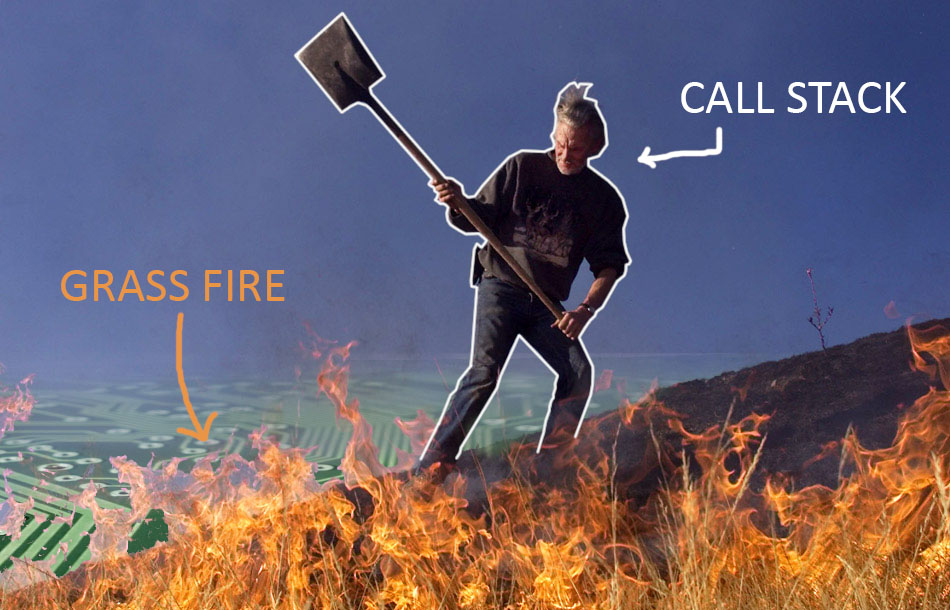
\includegraphics[width=0.6\linewidth]{figure/Analysis/firefighter.jpg}
	\caption{What happens inside your call stack during a grassfire algorithm. The fire spreads adding calls onto the stack, raging out of control, putting our call stack, the old man, in danger. Until the fire is done spreading the stack cannot resolve. When done spreading the call stack is resolved, represented by the old man, can out the fire.}
	\label{fig:firefighter}
\end{figure} 
Because of the relatively small blobs in our program, usually somewhere between 150 and 450 pixels, all we had to do prevent stack overflow was to increase the stack heap size to 4 mb instead of the visual studio standard of 1 mb. However larger resolutions would cause significantly bigger issues. If we double the number of pixel in each axis, we get a four times larger blob. At large camera sizes, the stack would have to be larger to accommodate the recursive function. Sampling that many pixels would also slow down the algorithm. While the webcam used in the prototype is tiny, early in the process it was thought that a larger resolution would be used in the final prototype. To anticipate this some options where added to the prototype. Namely the option to set a variable called \codeword{gridSize} which causes the algorithm to make jumps of size \codeword{gridSize} pixels instead of 1. Instead of checking the pixel to its right the algorithm will check the one \codeword{gridSize} to the right. Setting \codeword{gridSize} to 2 will cause the blobs to be four times as small, counteracting a larger camera resolution. Now the algorithms speed vs accuracy can be tailored to suit our specific need.
\subsection{Grassfire implementation}
Our implementation can be seen in listing \ref{listing:grassfireIm}. Due to its iterative nature, this method will be called many thousand times. Note that the function does not make use of the very computationally expensive Mat.at<uchar>(y,x) function. Instead we use pointers to navigate both horizontally and vertically.
\begin{figure}[H]
	\centering
	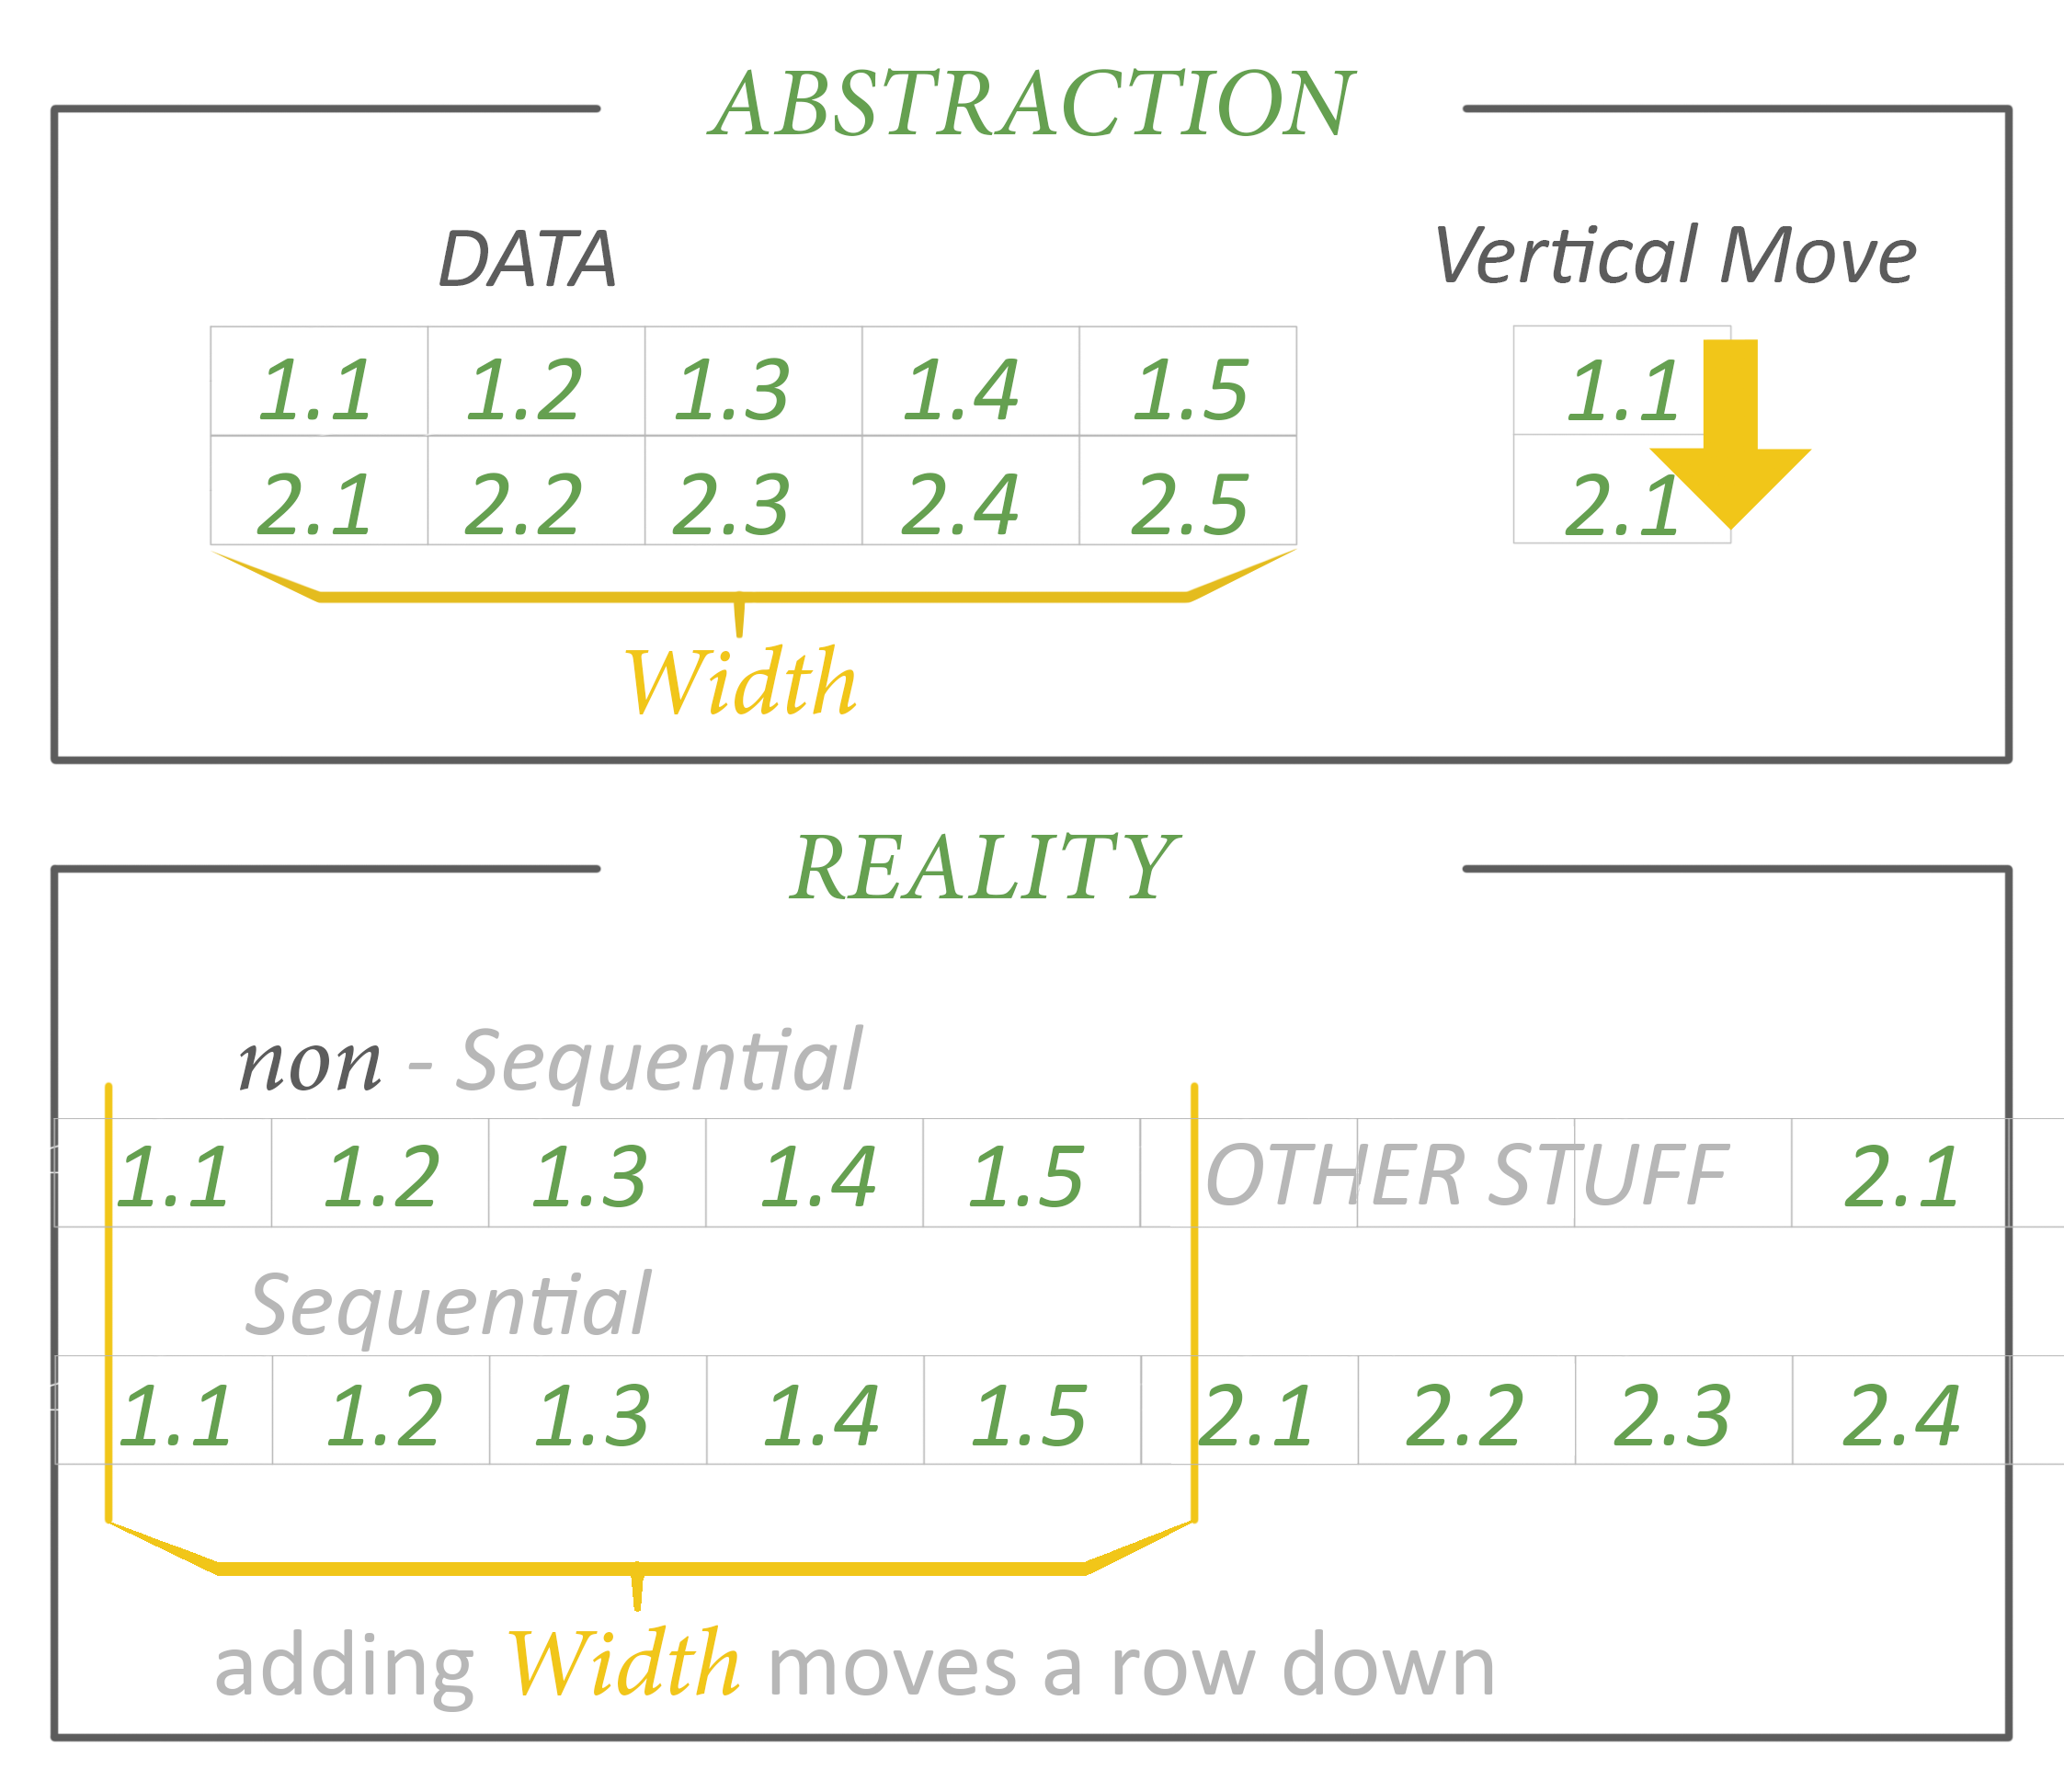
\includegraphics[width=0.6\linewidth]{figure/Analysis/data.png}
	\caption{Visualization of what happens when one adds the images width to a pointer. In a non-sequential image jumping doing this might result in writing to an invalid location. But in a sequentially laid out image it will result in the pointer pointing to the same index in the row below } 
	\label{fig:vis}
\end{figure}
 The implemented method only works if the data in the image is laid out sequentially. Being sequential means that the data of each row is laid out right after each other. So after the last index in the first row, comes the first index in the second row. Normally to get from a coordinate $(x,y)$ to $(x,y+1)$ one would have to get a pointer to the first column using the mat.ptr<uchar>(y+1) and then adding the x value to it. This is exactly what the Mat.at<uchar>(y,x) does. But if the image is sequential one can add the image width to its index and end up in the row below it, as illustrated in Figure \ref{fig:vis}.\\\\
 
 Now that we can navigate between pixel it is possible to implement the algorithm, and we implemented it as seen in listing \ref{listing:grassfireIm}
\begin{listing}[H]
	\caption{The drop fire function starts from one white pixel changes its color and recursively spreads until the entire blob has been consumed. It does this through connected component analysis, analyzing its connected pixels, and spreading to them if they are white.}
	\begin{minted}[frame=lines, framesep=2mm,baselinestretch=1.1,fontsize=\footnotesize,linenos]{c++}
void dropFire(uchar * pixel, glyphObj &store, int &width, int y, int x, cVector &from) {
	*pixel = store.nr;
	from.x = x;
	from.y = y;
	store.list.push_back(from);
	if (*(pixel + GRIDSIZE) == 255) {
		dropFire(pixel + GRIDSIZE, store, width, y, x + GRIDSIZE, from);
	}
	if (*(pixel + width) == 255) {
		dropFire(pixel + width, store, width, y + GRIDSIZE, x, from);
	}
	
	if (*(pixel - GRIDSIZE) == 255) {
		dropFire(pixel - GRIDSIZE, store, width, y, x - GRIDSIZE, from);
	}
	
	if (*(pixel - width) == 255) {
		dropFire(pixel - width, store, width, y - GRIDSIZE, x, from);
	}
}
	\end{minted}
	\label{listing:grassfireIm}
\end{listing} 
The arguments consist of a pointer to the pixel, the blob that this fire is going to add data to, and the image's width. Two ints that are the fire's current coordinates. A reference to a vector to avoid instantiating a new one in each recursion. The function starts on line 2 by changing the pixels color, in order to avoid infinite recursion. Lines 3 to 5 adds the current coordinates to the blob. Next are four if statements. Each check if the neighboring pixel in a certain direction are white. If any of them are, it spreads the fire in those directions with the new x and y values.\\
With the knowledge of how to create the grassfire and how it works, all we need is to find the white pixels where the fire should start.

\subsection{Scanning for white pixels}
First one loops through each pixel in the image and checks if it is completely white. Obviously this only works if the image is binary. In our case, the image is 8bit greyscale to help visualize the blobs for us humans. If the pixel is white, create a blob, add it the list of blobs, and start the fire at the pixel. This is implemented as shown in Listing \autoref{listing:grassfire}.
\begin{listing}[H]
	\caption{"We didn't start the grassfire". This algorithm did. It scans for white pixels, creates blobs if it finds any, and then starts fires}
	\begin{minted}[frame=lines, framesep=2mm,baselinestretch=1.1,fontsize=\footnotesize,linenos]{c++}
void grassFireBlobDetection(Mat &biImg, vector<glyphObj> &blobs) {
	int nRows = biImg.rows;
	int nCols = biImg.cols;
	int rowSize = nCols * GRIDSIZE;
	uchar * p;
	uchar * passer;
	glyphObj currentBlob;
	cVector assigner;
	int col = 245;
	for (int i = GRIDSIZE + 1; i < nRows - GRIDSIZE - 1; i += GRIDSIZE) {
		p = biImg.ptr<uchar>(i);
		for (int j = GRIDSIZE + 1; j < nCols - GRIDSIZE - 1; j += GRIDSIZE) {
			if (p[j] == 255) {
				blobs.push_back(currentBlob);
				blobs.back().nr = col;
				passer = &p[j];
				dropFire(passer, blobs.back(), rowSize, i-BORDER, j-BORDER, assigner);
				col -= 10;
				if (col < 20) {
					col = 245;
				}
			}
		}
	}
}
	\end{minted}
	\label{listing:grassfire}
\end{listing}
The arguments for this function are a reference to an binary image, and references to a vector of blobs that will be filled with the data. The \codeword{dropFire} function in Listing \ref{listing:grassfireIm} needs to be passed the images width. a variable for this is instantiated on line 4. A temporary blob object(currentBlob) vector(assigner), and uchar pointer(passer) is created to avoid instantiating these objects in the recursive function. A reference to these will be passed instead. Finally the fire's color is set to be 245 in line 9 since it should not be white(255). Inside the double for loop it checks if the current pixel is completely white. If it is, a new blob is added to the vector of glyphObject that contains the blobs it color is set to the value of col, and the fire starts. To make it easier to display which pixels that belong to which blob, the color is made darker. This means that different fire will "burn" different colors into the image. To prevent the color from becoming negative it is reset when it becomes to dark, in line 20 to 23.\\
\begin{figure}
	\centering
	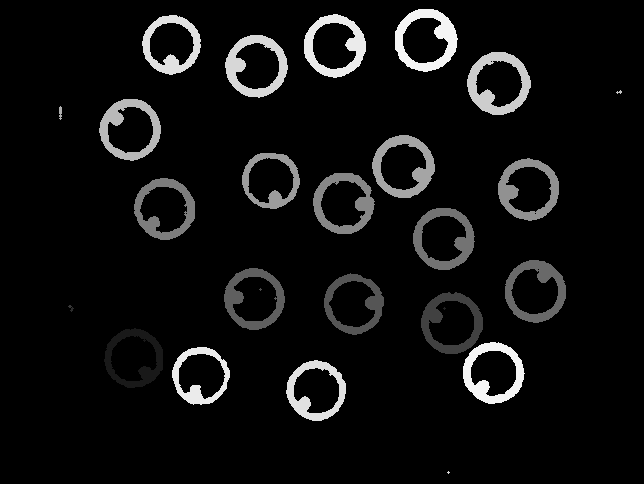
\includegraphics[width=0.6\linewidth]{figure/Analysis/grassfire.png}
	\caption{The test image after the grassfire algorithm has been run. Each blob is made slightly darker than the lost one, until a threshold where the color is made quiet white again}
	\label{fig:grsnapshot}
\end{figure} 
The results of the image before and after this algorithm has been run can be seen in Figure \ref{fig:grsnapshot}. It can be seen that each blob has been segmented from the difference in colors between them. As the color of the fire is changed each time a new fire is started. Now that we have a list of the pixels inside each blob, it is time to calculate the parameters are used to determine and evaluate the object.
\section{Blob analysis}
In this section we will deal with how to calculate parameters for a given blob, and how these are used to evaluate whether the blob is one of the markers.
\subsection{Parameter overview, and flow }
At present we have a list of the pixels in each blob. To evaluate the markerhood of a given blob it needs the following parameters.
\begin{enumerate}
	\item Number of pixels in the blob.
	\item Height to width relationship of the bounding box.
	\item Bounding box center.
	\item Rotation of the blob.
\end{enumerate}
When all parameters are acquired, and if the blob passes all the tests, it is time to check the value in the glyph. To do this, vectors are calculated based on the rotation that sample a pixel in each "bit" in the glyph and calculate the total value of it. If this value is between 1 and 255 it is considered a marker, and this blob is flagged so it can be sent to unity.\\\\

The flow of the algorithm can be seen in the flow chart below.
\todo{make a flow chart for this}
\\\\
In regards to calculating the parameters, some of them are very simple to find. Finding the size a blob is easy because \codeword{vector<type>} already contains a \codeword{.size()} method. The bounding box consist of looping through all coordinates and saving the smallest and largest x and y that the program encounters. Finding the center consists of averaging the same values for x and y respectively. Rotation, on the other hand is trickier and requires use of knowledge about the layout of the marker.  
\subsection{Rotation}
Finding a circle's rotation is impossible if it does not have any distinguishing features. So we added one, in the form of a small line towards the center that we call the direction line(seen to the left in Fig \ref{fig:vector}). If the center's coordinates are known, one can find the pixel in the blob closest to it. This pixel will be in the direction line. The distance from the center to the closest pixel will give create a vector, from which the rotation can be calculated. This method of finding rotation is the primary reason why we used the bounding box center over center of mass when finding the center. The center of mass would be shifted towards the rotation line, and therefore the direction vector will be less stable, as seen in Figure \ref{fig:boundbox}.\\
\begin{figure}
	\centering
	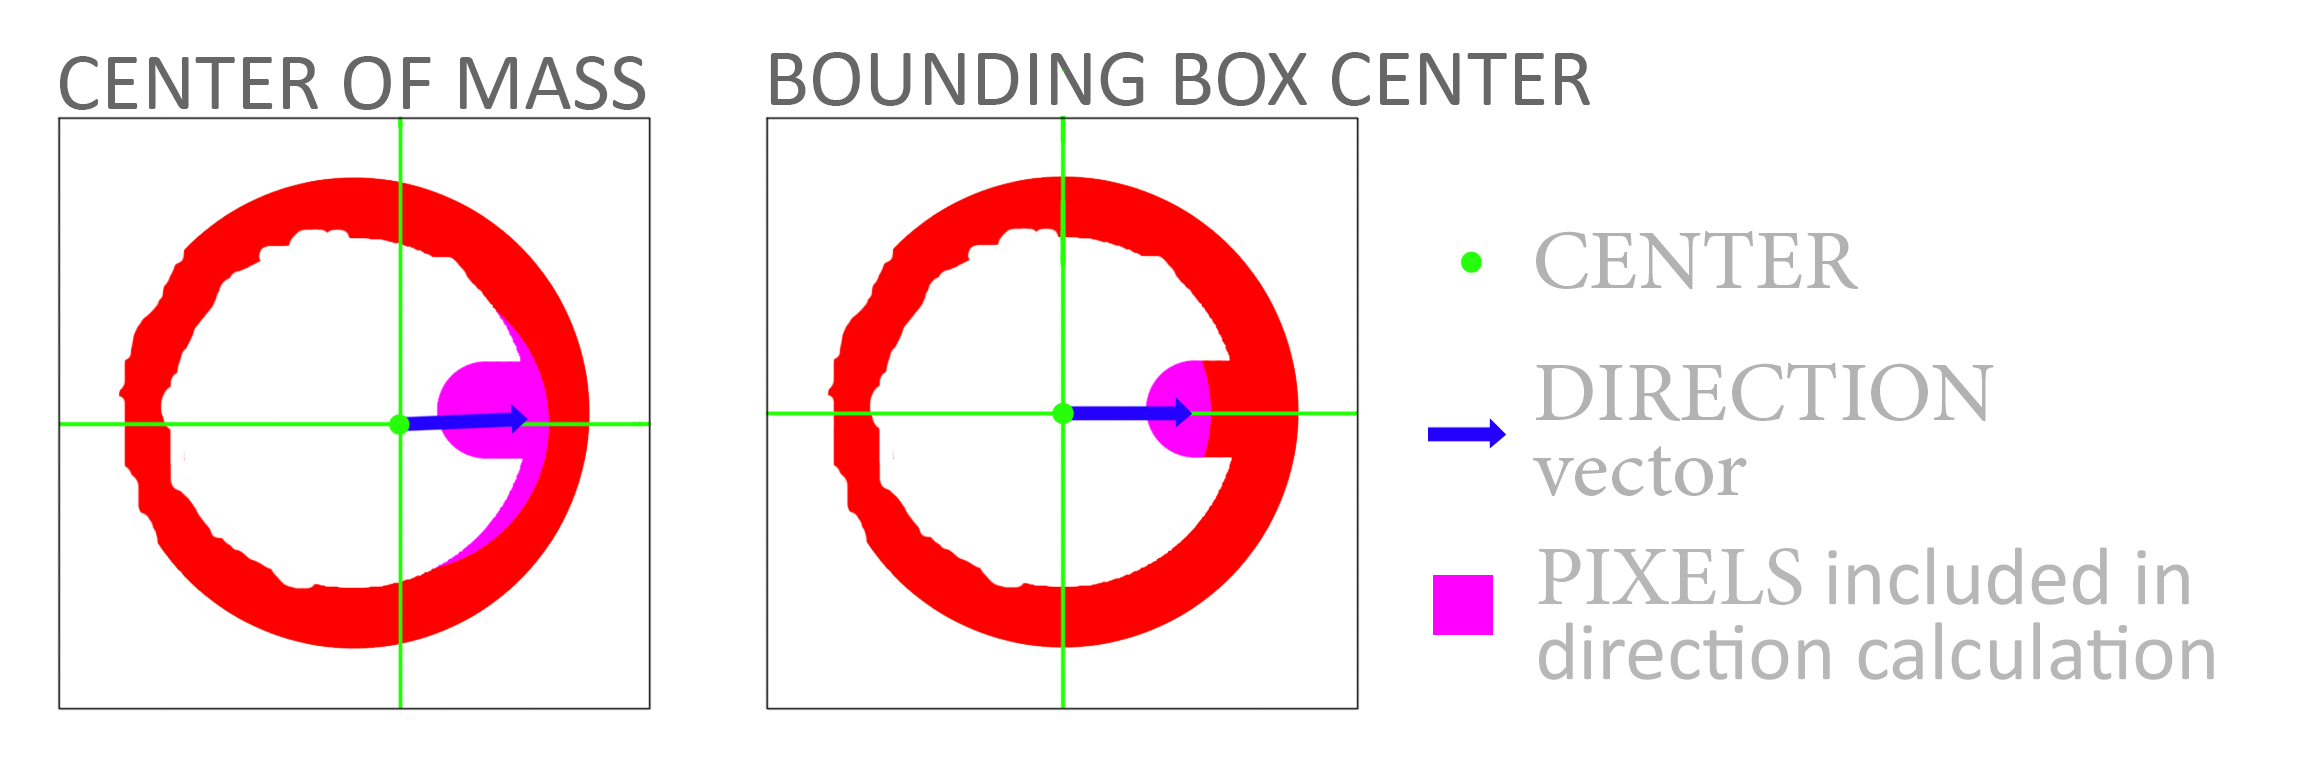
\includegraphics[width=1\linewidth]{figure/Analysis/boundingbox.png}
	\caption{the difference between using the center of mass or bounding box to find the blob center. With bad thresholding the found center is closer to the actual center, resulting in a better direction vector} 
	\label{fig:boundbox}
\end{figure}
We found that smaller blobs would have a more wobbly direction vector, because the direction line now contains fewer pixel. Since it only finds one pixel it could result in a drastic snap. To combat this, instead of only using the closest pixel we average all the pixel within 70\% of the circles radius. This allows us to average a bunch of pixels in the direction line without sampling any from the
periphery. Rotation is also calculated as a float instead of integer. These changes make the direction vector much more stable, and have been illustrated in Figure \ref{fig:lowpixel}
\begin{figure}
	\centering
	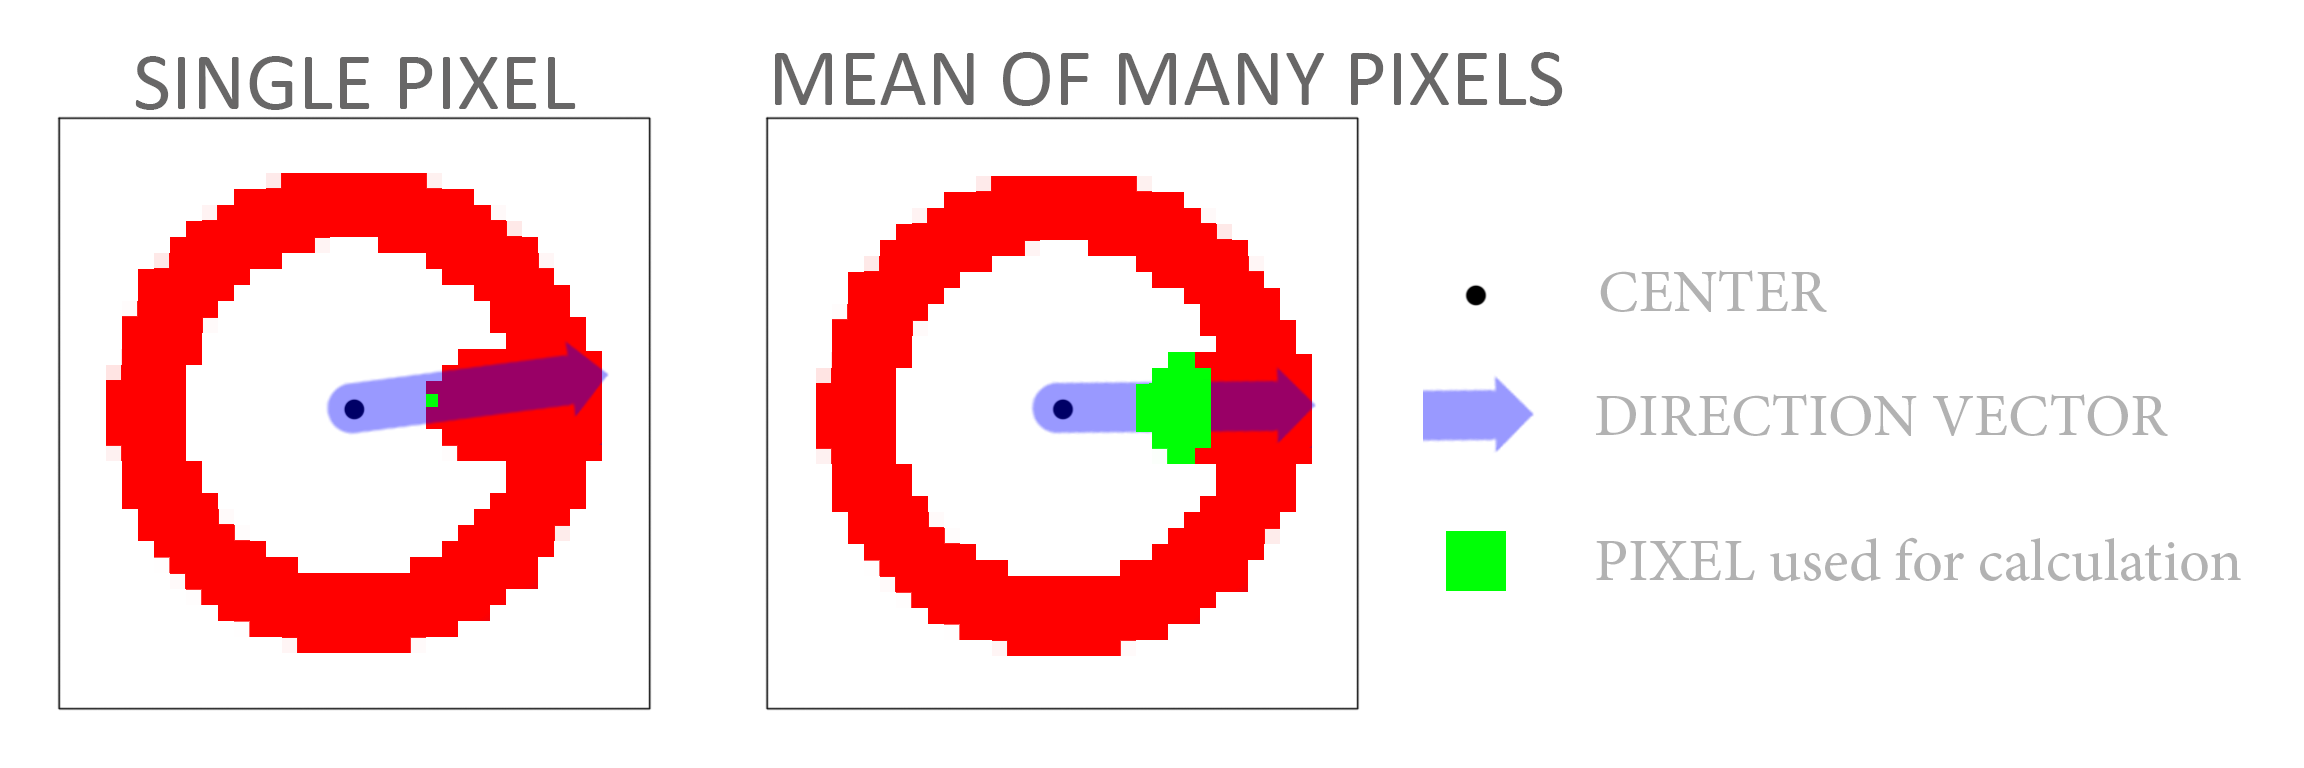
\includegraphics[width=1\linewidth]{figure/Analysis/lowpixel.png}
	\caption{illustration of the advantage of using mean of many pixel vs single closest pixel to calculate the direction vector.} 
	\label{fig:lowpixel}
\end{figure}
 The code, seen in listing \ref{listing:direction}, executes inside a loop through the list of blobs, and happens right after the bounding box and its center has been found. \codeword{i} refers to the current blob.
\begin{listing}[H]
	\caption{Direction vector calculation}
	\begin{minted}[frame=lines, framesep=2mm,baselinestretch=1.1,fontsize=\footnotesize,linenos]{c++}
float heightWidth = ((largestX - smallestX) / (float)(largestY - smallestY));
//check: discriminate based on height width relation
if (heightWidth > (1 + discrimHW) || heightWidth <(1 - discrimHW)) { continue; }	

radiusDist = (largestX - smallestX + largestY - smallestY) / 4;
searchDist = (float)radiusDist*0.70 * (float)radiusDist*0.70;
int dist;
vector<cVector> points;  //contains the pixels within 0.7 radius
//find pixel within search dist
for (auto &v : i.list) {	//loop through all pixels in the
	dist = (v.x - i.center.x) * (v.x - i.center.x) + (v.y - i.center.y) * (v.y - i.center.y);
	if (dist < searchDist) {
		points.push_back(v);
	}
}
float rotX = 0;
float rotY = 0;
for (auto &p : points) {
	rotX += p.x - centerX;
	rotY += p.y - centerY;
}
rotX = (rotX / points.size());
rotY = (rotY / points.size());
	\end{minted}
	\label{listing:direction}
\end{listing}
Now that a direction vector has been found, we need to calculate the the position of each bit fields on the marker. This is done with a bit of vector math and knowledge of the marker layout. A legend of the important components can be seen in Figure \ref{fig:vector}.
\subsection{Vectors to find sample points}
The direction vectors length will vary a bit, because sometimes the middle point moves a pixel or two. Under these circumstances the direction vector will still be reasonably stable, but its length will change depending on how much of the direction line is used for the direction calculation. Ideally one would like to base the vectors on a more stable property of the marker. For this reason, the direction vector is scaled so that its length is equal to the radius. We can now define distances as percentages of the markers radius. Sample points are the point where we check image intensity to determine whether the field is white or dark. These can be thought of as points on a "skeleton" made up of different vectors, as shown in Figure \ref{fig:vector}.
\begin{figure}
	\centering
	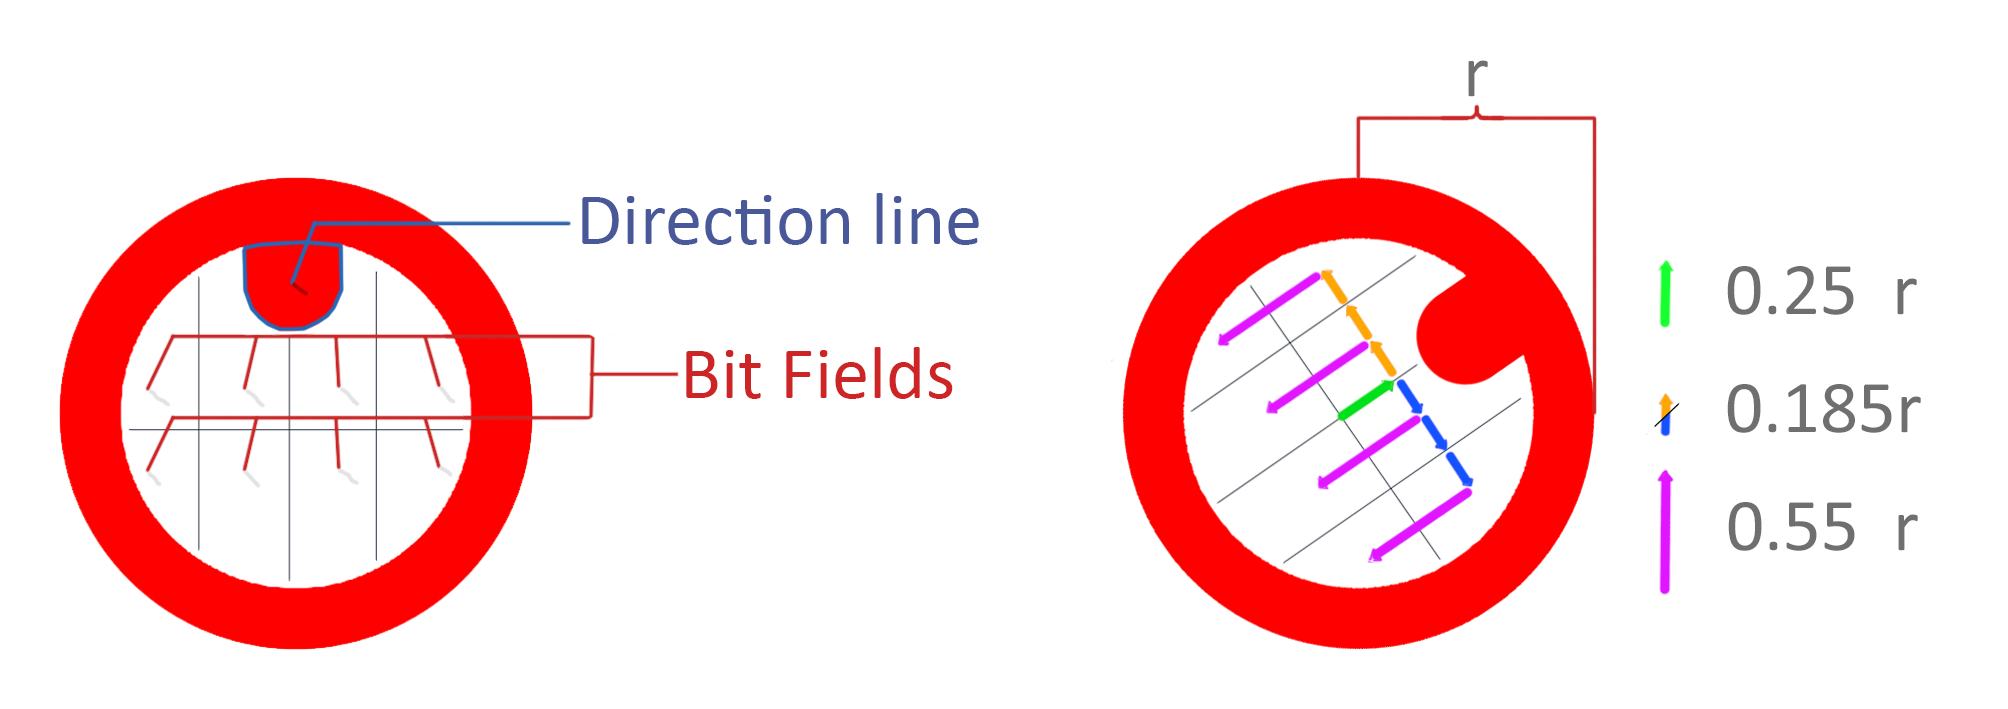
\includegraphics[width=1\linewidth]{figure/Analysis/vector.png}
	\caption{To the left one can see the location of the direction line, used to find the direction that the marker is facing, and the bit fields used to ascertain the marker's value. To the right, the "skeleton" of vectors used to find bit fields coordinates are shown.} 
	\label{fig:vector}
\end{figure}
Finding the sample points is a matter of adding the correct vectors to the marker's center. To begin a start point is created 25 percent towards the direction line. From here there are three different type of vector used to reach the sample points. Two that move perpendicular to the direction, used to move "sideways", and one that moves opposite the direction to get the second row of points. Rotating a vector 90° is fortunately easy, and can be done by flipping the axis and changing a sign(- x, or -y).    
\begin{listing}[H]
	\caption{Declaration of vectors used to find sample points}
	\begin{minted}[frame=lines, framesep=2mm,baselinestretch=1.1,fontsize=\footnotesize,linenos]{c++}
	int startPointX = centerX + rotX*0.25;
	int startPointY = centerY + rotY*0.25;
	
	//Perpendicular movement
	float cClockX = -rotY*0.185;
	float cClockY = rotX*0.185;
	float clockX = rotY*0.185;
	float clockY= -rotX*0.185;
	
	//Backwards movement
	float reverseX = -rotX*0.55;
	float reverseY = -rotY*0.55;
	\end{minted}
	\label{listing:vectors}
\end{listing}
From these the sample points can be acquired. Once they have all there is left is to check whether the bit fields that they point to are dark or white. This is done by checking each color in the original image and, if they all are below a threshold, adding 2 to the power of the field to the total count. The implementation can be seen in Listing \ref{listing:sumingval}.
 \begin{listing}[H]
 	\caption{After finding the sample points, this code checks the value in that pixel and, if low enough, adds it's value to the bit counter. If the bit counter is larger than 0, when all points have been checked, the bit counter is assigned to the blob's nr, allowing it to be returned to unity.}
 	\begin{minted}[frame=lines, framesep=2mm,baselinestretch=1.1,fontsize=\footnotesize,linenos]{c++}
int bitCounter = 0;					//total marker value
int thresh = 50;
for (auto &sp : searchPoints) {		//loop through each point
	Vec3b intensity = drawImg.at<Vec3b>(sp.y, sp.x);
	if (intensity[0]< thresh && intensity[1] < thresh && intensity[2] < thresh) {
		bitCounter += pow(2, iterations);
	}
}

if (bitCounter > 0) {
	i.returnable = true;
	i.nr = bitCounter;
}
 	\end{minted}
 	\label{listing:sumingval}
\end{listing}
Finally, since we often get 0 as a false positive from different skin blobs, we do not return the object to unity unless at least one of the bit fields are dark.
So finally we can present the final image after the blobs have been analyzed. 
\begin{figure}[H]
	\centering
	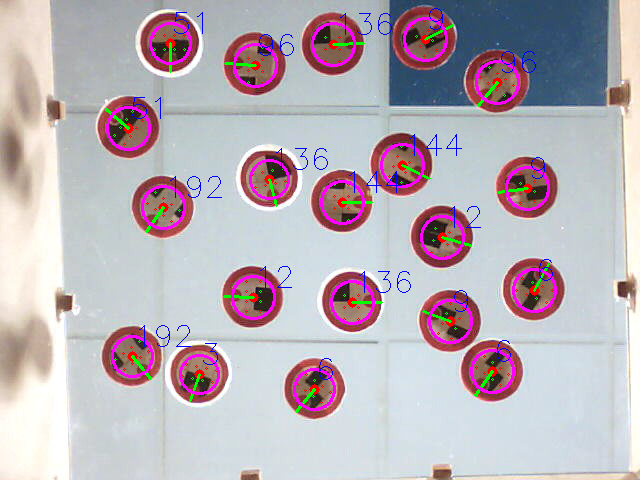
\includegraphics[width=1\linewidth]{figure/Analysis/output.png}
	\caption{The output after the blobs from the grassfire has been analyzed. The radius used to find points for the direction vector is drawn in purple. The direction vector after scaling it to have a length of radius is drawn in green. The sample points are drawn in either red, if they are too white, and green if they are considered dark} 
	\label{fig:output}
\end{figure}

Returning the objects to unity can be done very simply. 
 \begin{listing}[H]
	\caption{returning all blobs that have passed the test to unity}
	\begin{minted}[frame=lines, framesep=2mm,baselinestretch=1.1,fontsize=\footnotesize,linenos]{c++}
for (auto &blob : blobs) {
if (outDetectedMarkersCount == maxOutMarkersCount)	break;
if (blob.returnable == false)	continue;
rotation = acos(blob.rotation.x / sqrt((blob.rotation.x * blob.rotation.x) + (blob.rotation.y * blob.rotation.y)));
outMarkers[outDetectedMarkersCount] = ObjectData(screenWidth - blob.center.x, screenHeight - blob.center.y, blob.nr, blob.rotation.x, blob.rotation.y, (180 / 3.1415) * rotation);
outDetectedMarkersCount++;
}
	\end{minted}
	\label{listing:return}
\end{listing}
After all of that the data is now in unity and the image processing section is now now done.
\section{Limitations}
Or different section title. This section will describe how the implementation differs from the description of the original idea in the "Design" section. Why was it not possible to do X (e.g. live update or 1024 item types etc.) and what did we do instead?